\begin{document}
	
The Voltage regulator used was a LM7805. The voltage regulator is used because the CMOS ring oscillator and LED driver were designed to run on a source voltage of 5V. The power supply provided, however, is a 9V DC battery. The voltage, therefore, needs to be reduced. The voltage regulator operates by taking an input voltage and step it down to some lower voltage by shedding the difference in energy between the two potentials in the form of heat. Figure \ref{fig:voltageregulator} shows the circuit configuration for the LM7805.

\begin{figure}[H]
	\centering
	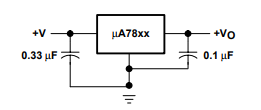
\includegraphics[width=0.5\linewidth]{CircuitDevelopment/voltageregulator}
	\caption[Voltage regulator]{Configuration of voltage regulator\cite{b4}}
	\label{fig:voltageregulator}
\end{figure}

The equivalent circuit model for the LM7805 is shown. Notably, the circuit was not included in simulations and was constructed during the Implementation phase.

	
	
	
	
	
\end{document}